\chapter{Results} \label{cha:results}
TODO: Overview of results chapter.

% 800 Office woman

\iffalse
\begin{figure}[h]
  \centering
  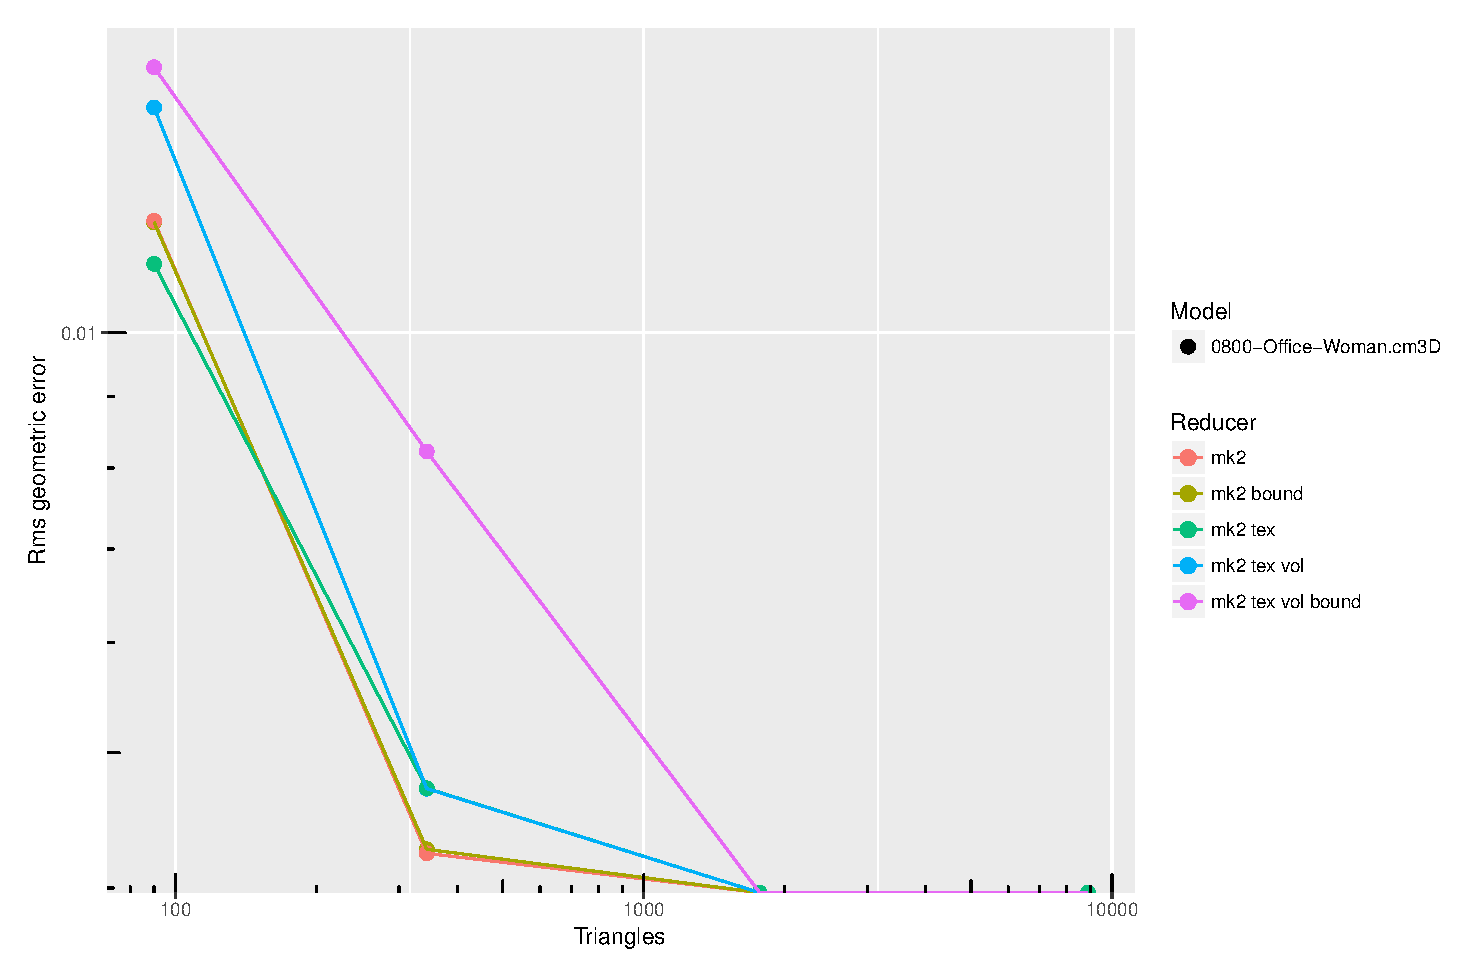
\includegraphics[width=\textwidth]{figures/Rdata/geometric_800.eps}
  \caption{Rms geometric error of ``office woman'' model}
  \label{fig:woman_geometric_error}
\end{figure}


\begin{figure}[h]
  \centering
  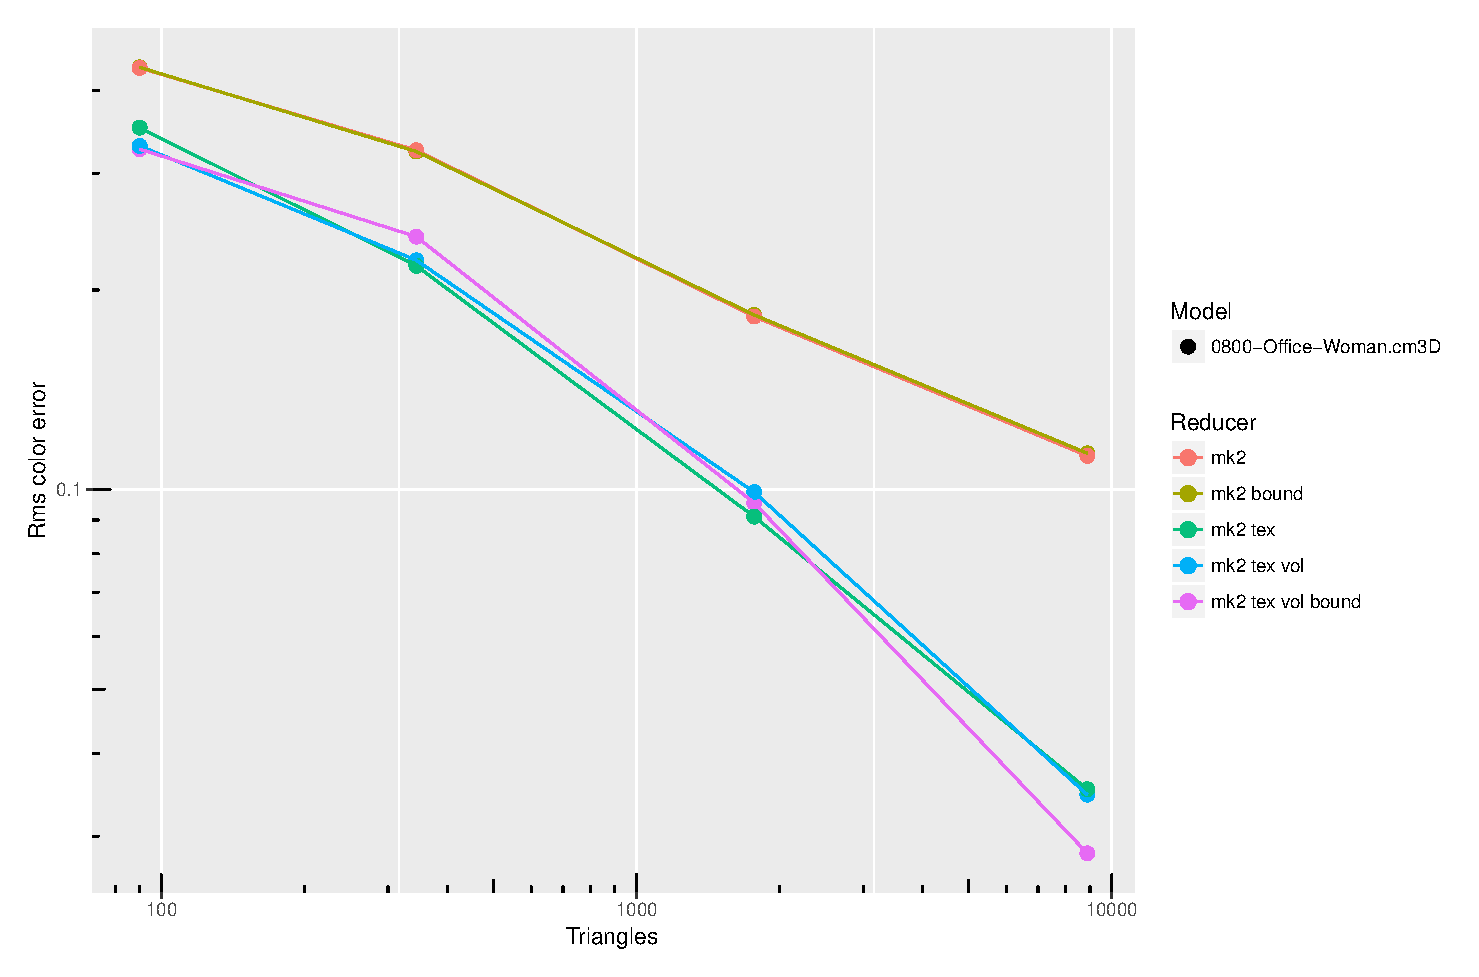
\includegraphics[width=\textwidth]{figures/Rdata/color_800.eps}
  \caption{Rms color error of ``office woman'' model}
  \label{fig:woman_color_error}
\end{figure}
\fi

\section{RMS luminance error}
RMS luminance error was computed by rendering multiple images of a model from multiple angles and can be seen in \cref{fig:mean_luminance_error}. Four LoD:s are presented where \emph{super} have the most amount of triangles and \emph{low} have the least amount of triangles. The error was measured for different settings of seam and volume preservation.

\begin{figure}[h]
  \centering
  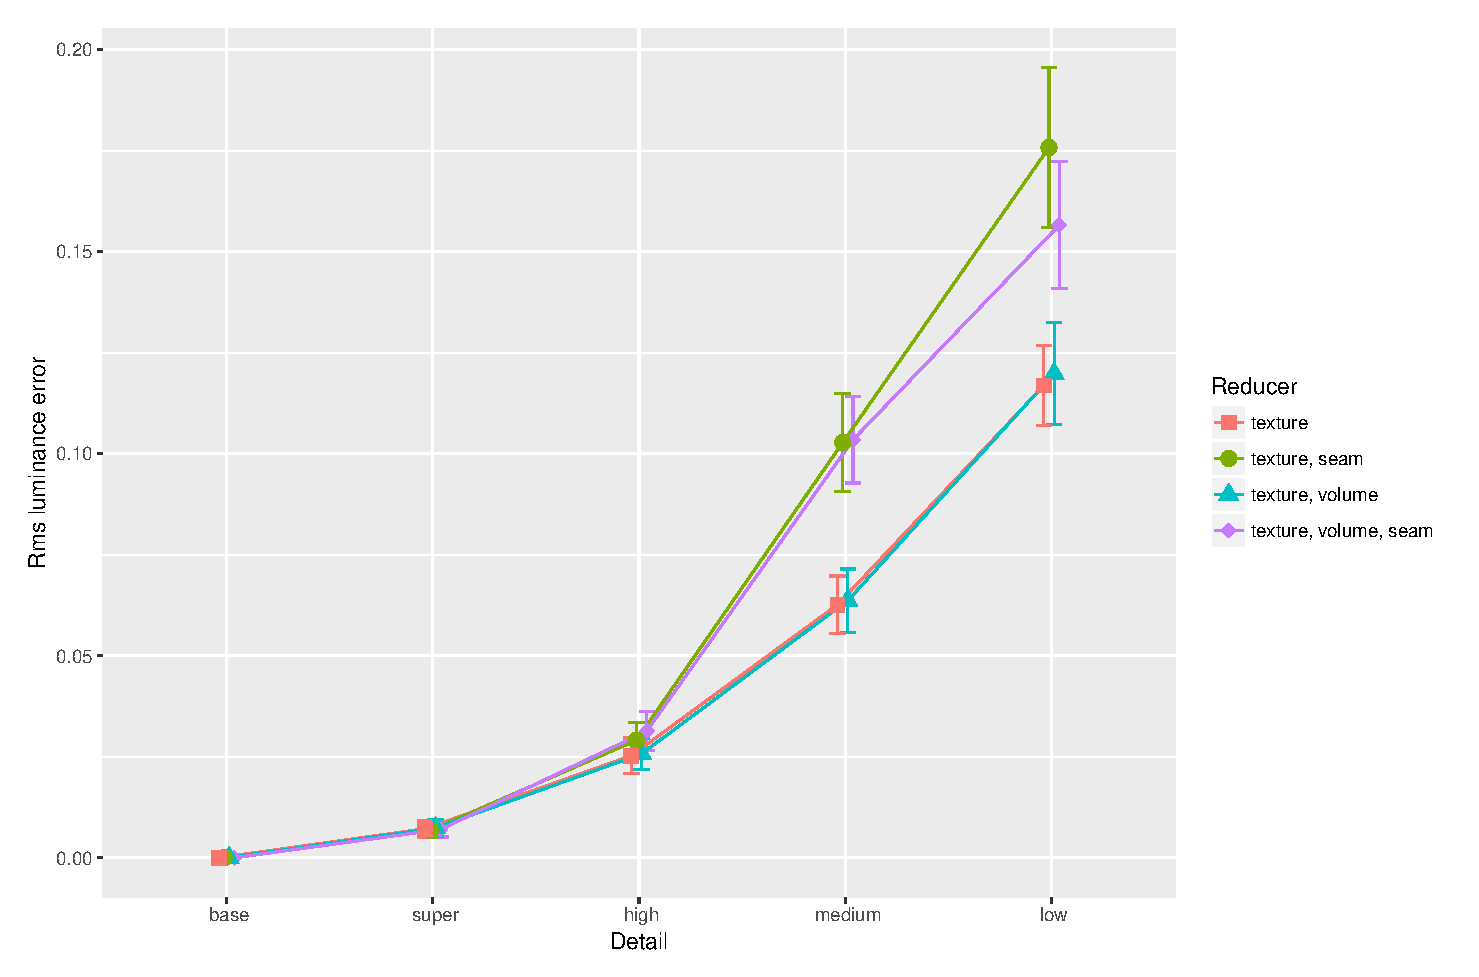
\includegraphics[width=\textwidth]{figures/Rdata/rms_luminance.eps}
  \caption{Rms luminance error}
  \label{fig:mean_luminance_error}
\end{figure}

\section{Hausdorff distance}

\section{Improved Texture}
A pull-push algorithm was implemented in order to improve the texture that is used by a mesh since undefined areas may be used. Given a texture (\cref{fig:original_texture_atlas}), rays are casted for each pixel in order to generate a black and white image. Valid pixels get a white color and invalid pixels a black color as seen in \cref{fig:valid_pixels}. Pixels with a corresponding black pixel will be filled in by the pull-push algorithm. This will result in the texture seen in \cref{fig:improved_texture} where all the empty pixels have been filled in.

\begin{figure}[h]
  \centering
  \begin{subfigure}[b]{.3\textwidth}
    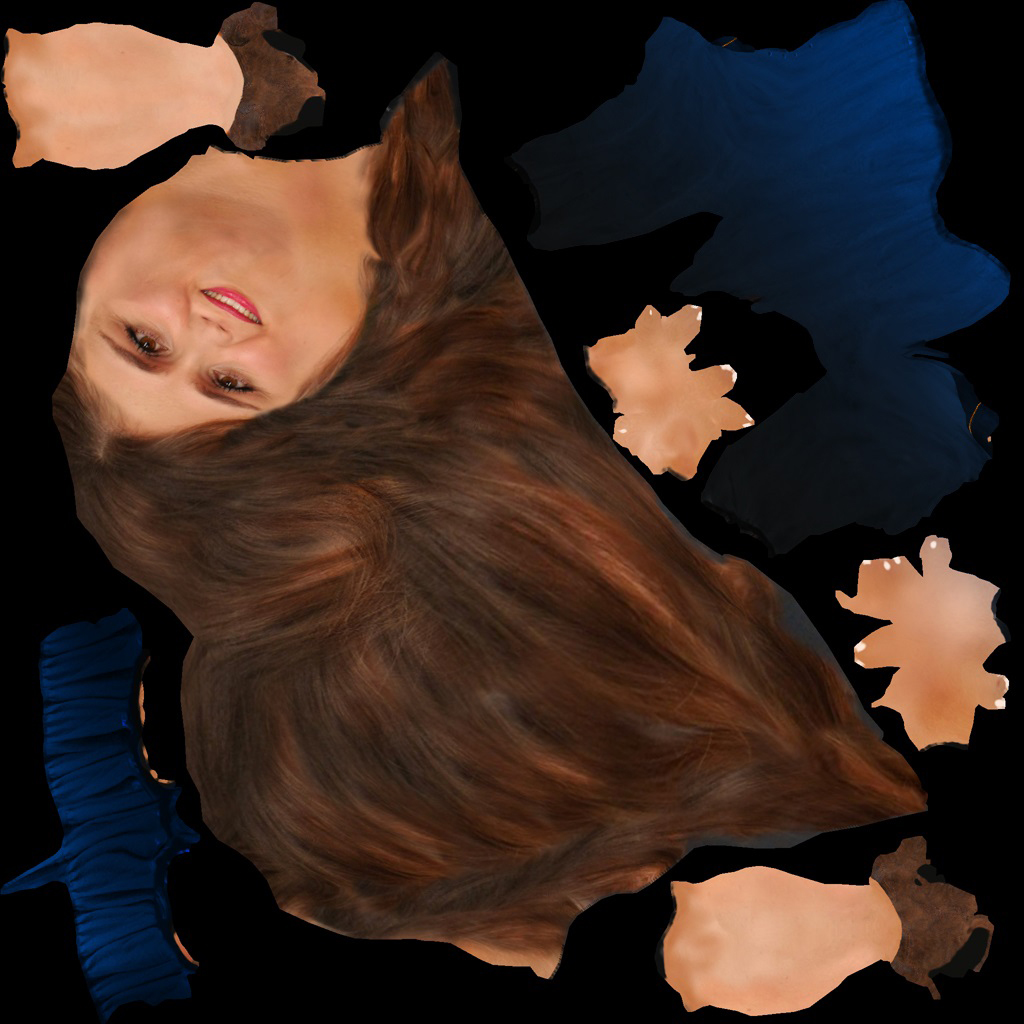
\includegraphics[width=\textwidth]{figures/woman_input.jpg}
    \caption{Original}
    \label{fig:original_texture_atlas}
  \end{subfigure}
  ~
  \begin{subfigure}[b]{.3\textwidth}
    
\includegraphics[width=\textwidth]{figures/woman_bound.png}
    \caption{Valid pixels}
    \label{fig:valid_pixels}
  \end{subfigure}
  ~
  \begin{subfigure}[b]{.3\textwidth}
    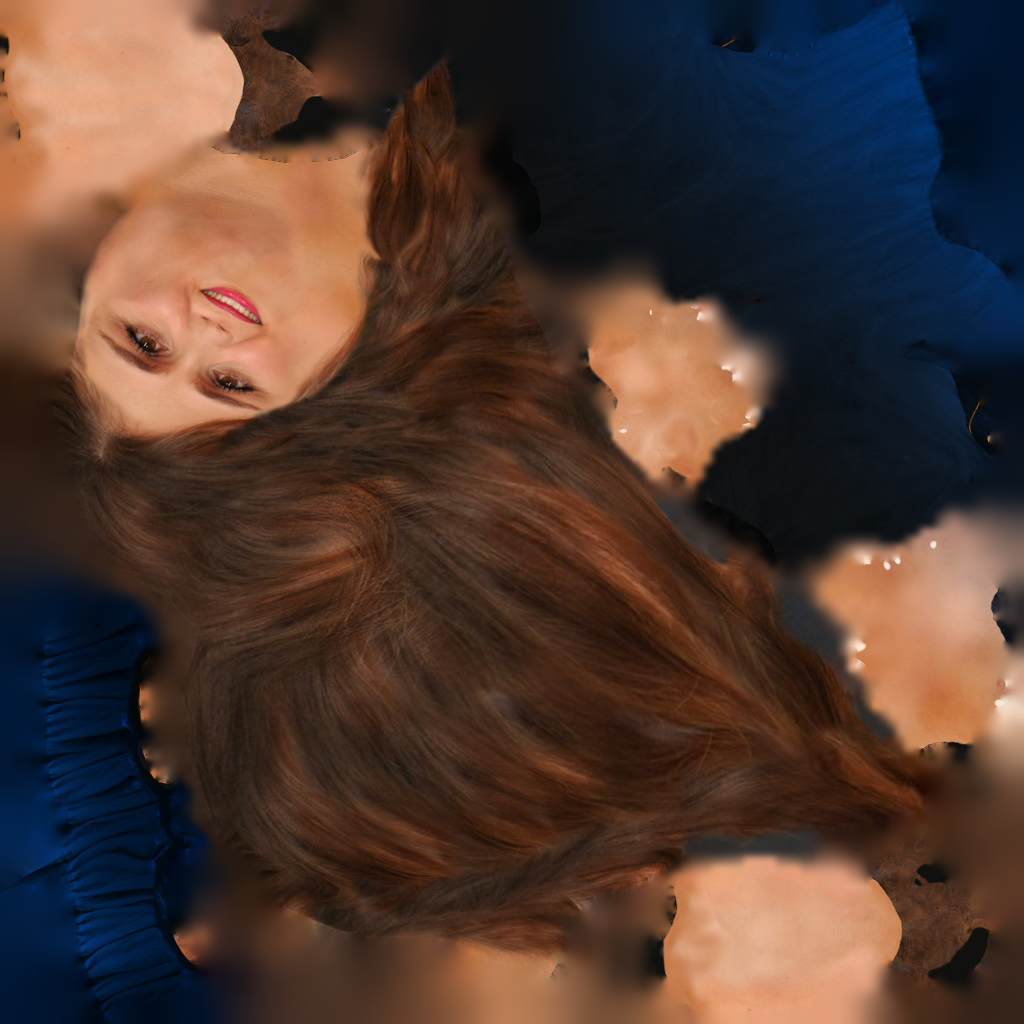
\includegraphics[width=\textwidth]{figures/woman_output.png}
    \caption{Improved texture}
    \label{fig:improved_texture}
  \end{subfigure}
  \caption{Filling in empty pixels in the texture atlas}
  \label{fig:improve_texture_atlas}
\end{figure}

Simplification of the office woman model introduce some black areas where the original seam used to be (\cref{fig:using_original_texture}). The same model have also been rendered with the new improved texture (\cref{fig:using_improved_texture}) to give a better appearance.

\begin{figure}[h]
  \centering
  \begin{subfigure}[b]{.2\textwidth}
    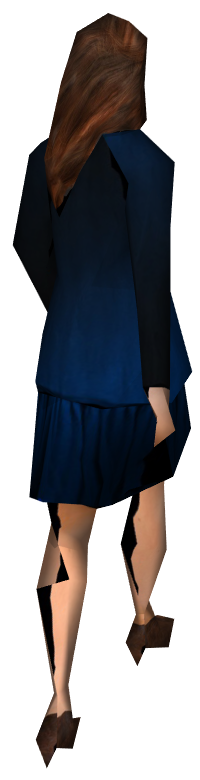
\includegraphics[width=\textwidth]{figures/woman_render.png}
    \caption{Using original texture}
    \label{fig:using_original_texture}
  \end{subfigure}
  \qquad
  \begin{subfigure}[b]{.2\textwidth}
    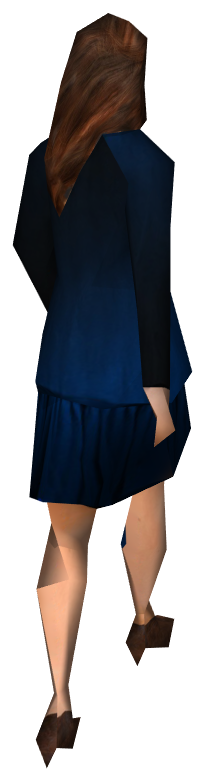
\includegraphics[width=\textwidth]{figures/woman_render_improved.png}
    \caption{Using improved texture}
    \label{fig:using_improved_texture}
  \end{subfigure}
  \caption{Mesh using original and improved texture}
  \label{fig:texture_comparison}
\end{figure}

% super:  8886
% high:   1768
% medium: 344
% low:    90

\begin{figure}[h]
  \centering
  \begin{subfigure}[b]{.22\textwidth}
    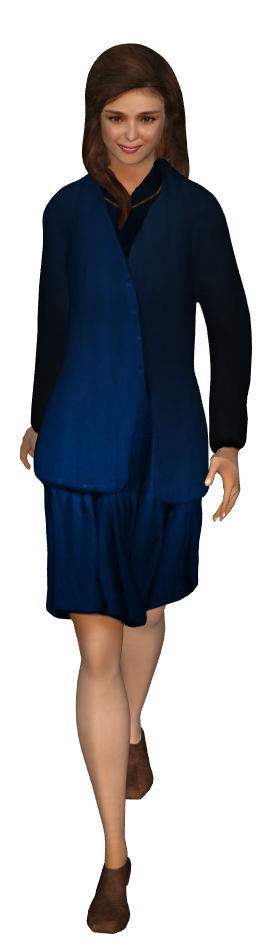
\includegraphics[width=\textwidth]{figures/woman/cropped/0.png}
    \caption{super}
    \label{fig:woman0}
  \end{subfigure}%\qquad
  \begin{subfigure}[b]{.22\textwidth}
    
\includegraphics[width=\textwidth]{figures/woman/cropped/1.png}
    \caption{high}
    \label{fig:woman1}
  \end{subfigure}
  \centering
  \begin{subfigure}[b]{.22\textwidth}
    
\includegraphics[width=\textwidth]{figures/woman/cropped/2.png}
    \caption{medium}
    \label{fig:woman2}
  \end{subfigure}%\qquad
  \begin{subfigure}[b]{.22\textwidth}
    
\includegraphics[width=\textwidth]{figures/woman/cropped/3.png}
    \caption{low}
    \label{fig:woman3}
  \end{subfigure}
  \caption{Office woman LoD:s}
  \label{fig:woman_lod}
\end{figure}


\begin{figure}[h]
  \centering
  \begin{subfigure}[b]{.22\textwidth}
    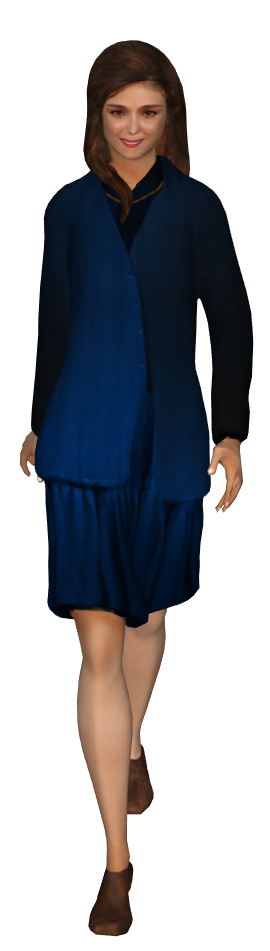
\includegraphics[width=\textwidth]{figures/woman/equal_distance/0.png}
    \caption{super}
    \label{fig:womaneq0}
  \end{subfigure}%\qquad
  \begin{subfigure}[b]{.22\textwidth}
    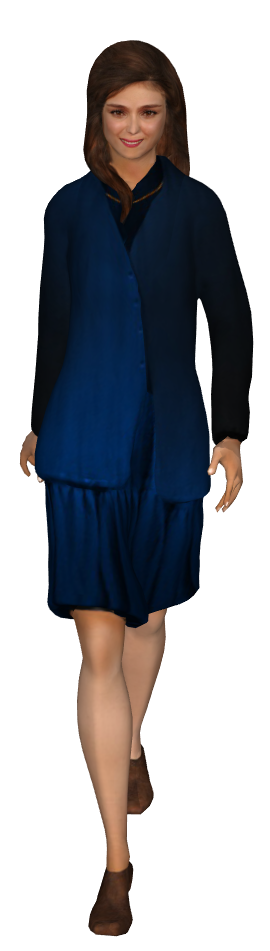
\includegraphics[width=\textwidth]{figures/woman/equal_distance/1.png}
    \caption{high}
    \label{fig:womaneq1}
  \end{subfigure}
  \centering
  \begin{subfigure}[b]{.22\textwidth}
    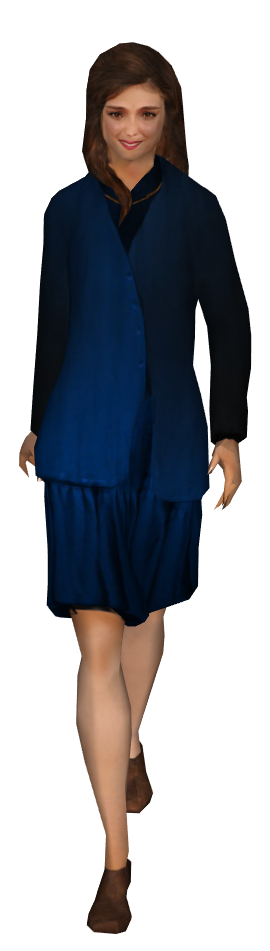
\includegraphics[width=\textwidth]{figures/woman/equal_distance/2.png}
    \caption{medium}
    \label{fig:womaneq2}
  \end{subfigure}%\qquad
  \begin{subfigure}[b]{.22\textwidth}
    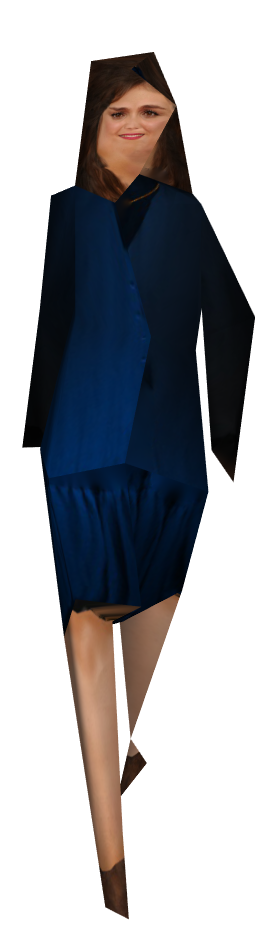
\includegraphics[width=\textwidth]{figures/woman/equal_distance/3.png}
    \caption{low}
    \label{fig:womaneq3}
  \end{subfigure}
  \caption{Office woman LoD:s}
  \label{fig:woman_lodeq}
\end{figure}
